\chapter{Simulação dos Ataques}
\label{chap:Simulacao}

	Nesta seção serão abordados tópicos relativos aos ataques realizados de um
	host atacante para um servidor vítima.

	Serão utilizados os alguns ataques e geradores de ruídos sugeridos por \cite{Morais}.
	Não serão implementados todos, pois, alguns deles só fazem sentido na rede
	em que os testes foram executados e não em qualquer ambiente. Os ataques e ruídos
	utilizados foram:

	\begin{itemize}
		\item Ping;
		\item Fingerprint;
		\item Footprint;
		\item Flood Attack;
		\item Brute Force.
	\end{itemize}

	\section{Geração de Ruído com Ping}
	\label{sec:Geracao_de_Ruido_com_Ping}
	Nesta geração de ruído, foi feito a partir do host atacante com ip 192.168.0.16
	utilizando o comando ping ipDaVitima. O comando utilizado pode ser visto na
	figura \ref{fig:ping_atacante} a seguir.


	\begin{figure}[h]
	 \centering
	 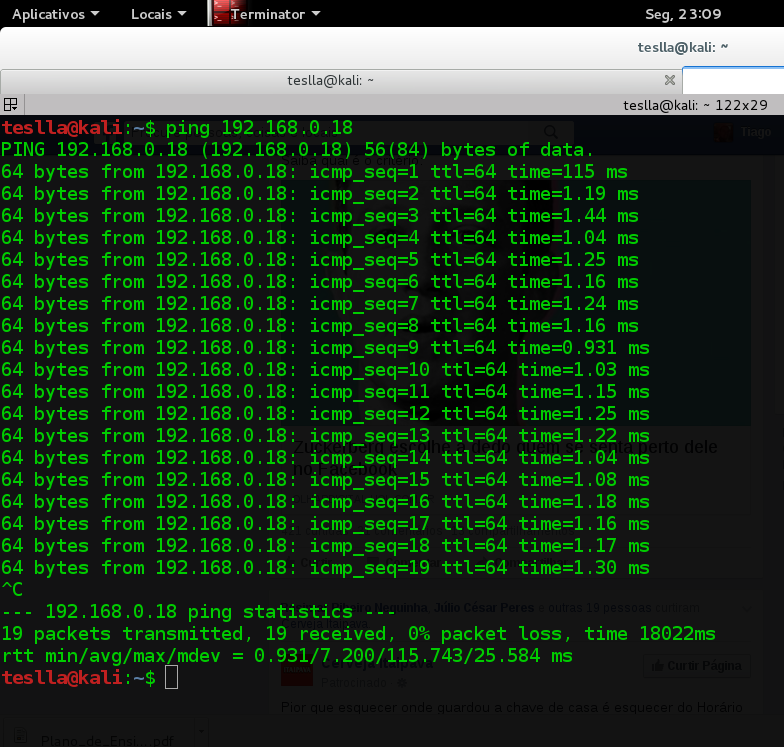
\includegraphics[width=300px, scale=1]{resource/ping_atacante}
	 \caption{Atacante - Envio de ping's para o servidor}
 \label{fig:ping_atacante}
 \end{figure}

Foram enviados 19 pacotes com intervalo de aproximadamente um segundo entre cada e
56 bytes de dado, sendo que todos foram recebidos.

 Todos os pacotes enviados para o servidor vítima são capitados pelo servidor
 que possui o sistema IDS/IPS instalado. A figura \ref{fig:ping_servidor} a seguir representa
 esta captura.

	\begin{figure}[h]
	 \centering
	 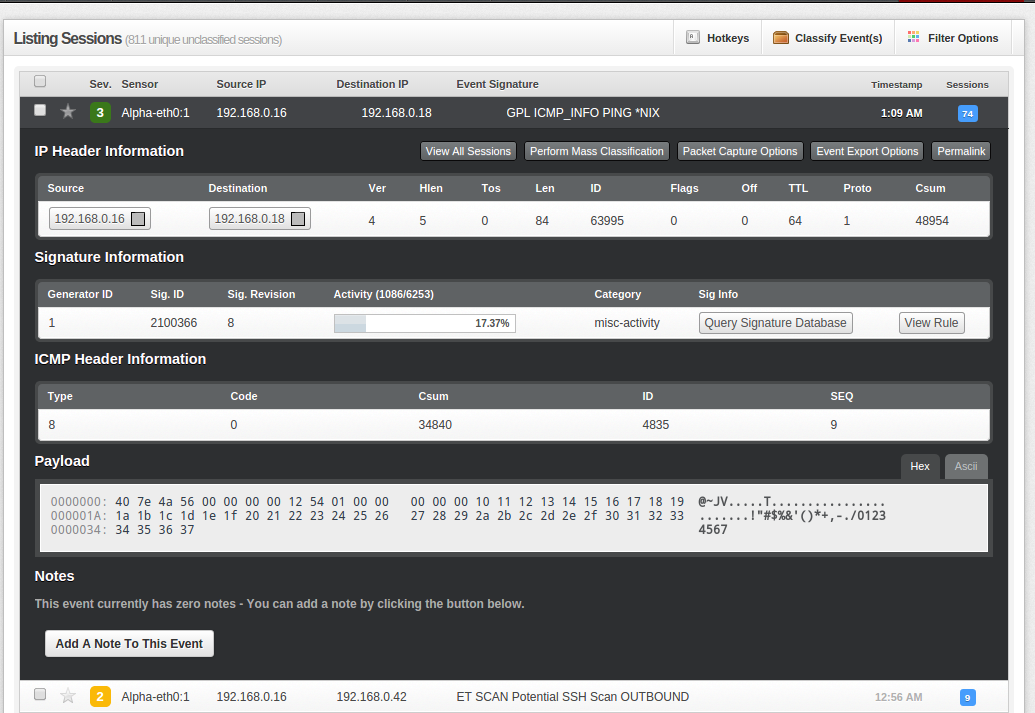
\includegraphics[width=400px, scale=1]{resource/ping_servidor}
	 \caption{Vítima - Detecção dos ping's solicitados pela vítima}
 \label{fig:ping_servidor}
 \end{figure}

 A figura \ref{fig:ping_servidor} apresenta vários dados dos pacotes capturados.
 Neste caso, há o nível de periculosidade da regra identificada, a interface de rede
 utilizada para a captura, no caso o Alpha eth0, endereços de IP de origem e destino,
 A mensagem transmitida pela regra, o pacote descrito em hexadecimal ou em
 Ascii, conforme a necessidade do usuário.

 A regra utilizada para capturar pacotes utilizado pela ferramenta ping
 foi demonstrada com a quantidade de pacotes recebidos. Neste caso, ela capturou
 74 pacotes, sendo que 19 foram deste último teste. O restante foram oriundos de ping's
 passados.

 \section{Geração de Ruído com Fingerprint}
Este passo, que consiste em varrer uma rede a procura de IP's válidos ao verificar
se uma determinada porta está aberta, gera um pouco de ruído para o servidor que é
captado pelo IDS/IPS.

É um procedimento bem simples que utiliza o comando: nmap redeAserEscaniada, neste
caso foi utilizado o comando:
\begin{framed}
 nmap 192.168.0.0/24
\end{framed}

Este foi utilizado para escanear todos os IP's entre
192.168.0.0 e 192.168.0.255, como pode ser visto na figura \ref{fig:atacante_varredura} a seguir.

	\begin{figure}[h]
	 \centering
	 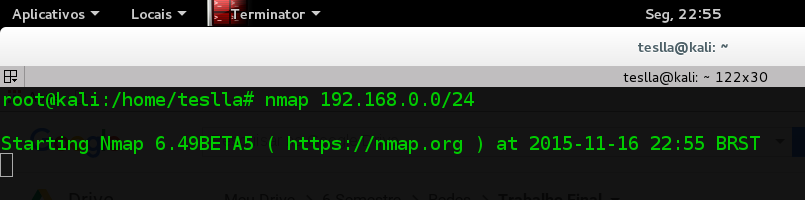
\includegraphics[width=300px, scale=1]{resource/atacante_varredura}
	 \caption{Atacante - Varredura de ip's válidos na rede 192.168.0.0/24}
 \label{fig:atacante_varredura}
 \end{figure}

O servidor com o Snort instalado observa a varredura feita na rede pelo atacante.
É possível observar que ele tentou conexões com vários serviços:

\begin{itemize}
	\item SSH na porta 22
	\item Oracle SQL na porta 1521
	\item PostgreSQL na porta 5432
	\item MSSQL na porta 1433
	\item mySQL na porta 3306
\end{itemize}


	 Além de ser indicado que uma varredura estava sendo executada. O alerta da mensagem:
	 ET SCAN Potential VNC Scan.

	 \section{Geração de Ruído com FootPrint}
	 \label{sec:Geracao_de_Ruido_com_FootPrint}
	 Esta geração de ruído consiste em um Port Scan Utilizado para identificar quais
	 portas estão abertas em um determinado IP, além de visualizar quais os serviços
	 que estão sendo providos e a versão.

	 A ferramenta utilizada para fazer o Port Scan foi a Zenmap, uma variação do nmap
	 com interface gráfica. Nela são passados os comandos para executar um scan
	 intensivo no IP da vítima, o exemplo utilizado na nossa varredura pode ser
	 visto na figura \ref{fig:atacante_port_scan}. Os comandos utilizados foram:

	 \begin{framed}
		 nmap -T4 -A -v 192.168.0.18
	 \end{framed}


	 \begin{figure}[h]
 	 \centering
 	 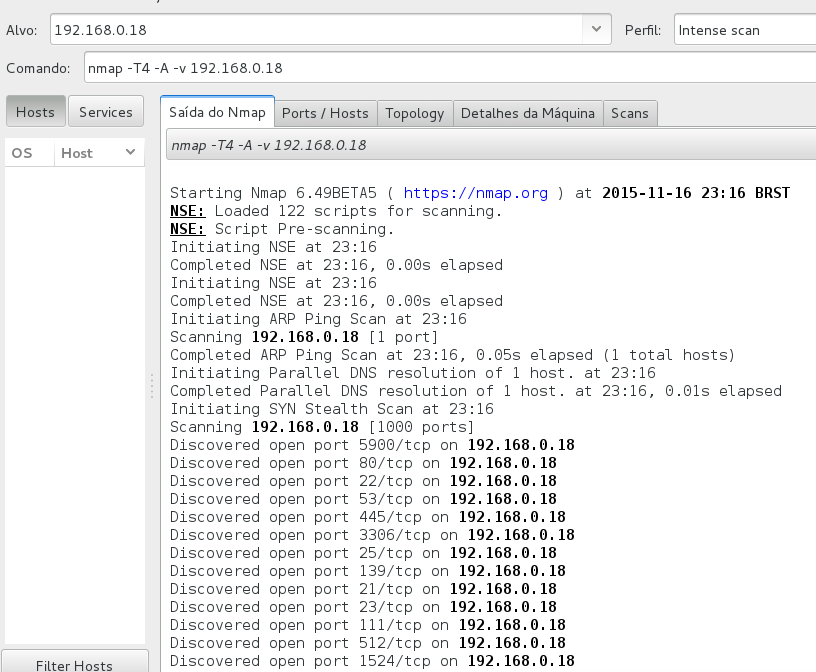
\includegraphics[width=350px, scale=1]{resource/atacante_port_scan}
 	 \caption{Atacante - Port scan Utilizando Zenmap}
  \label{fig:atacante_port_scan}
  \end{figure}

	Ao tempo em que a varredura ocorre, o servidor Snort verifica todas as tentativas
	de abertura de porta. Ele identifica também que está acontecendo uma varredura
	que utiliza o nmap como base. O log dos eventos capturados pode ser visualizado na
	figura \ref{fig:vitima_log_port_scan}.

	 \begin{figure}[h]
 	 \centering
 	 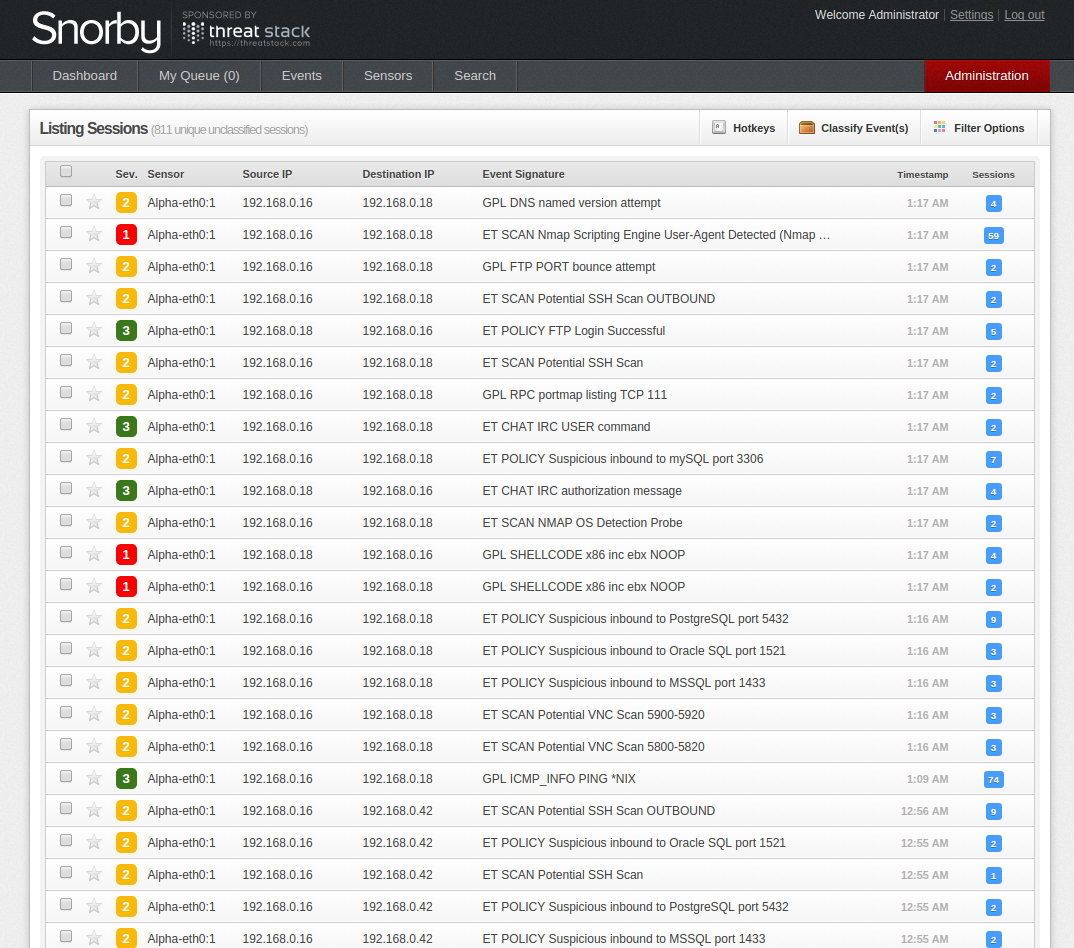
\includegraphics[width=400px, scale=1]{resource/vitima_log_port_scan}
 	 \caption{Vítima - Sequencia de Scans realizados pelo atacante de 1-16 até 1-17 am}
  \label{fig:vitima_log_port_scan}
  \end{figure}

	O servidor Identificou uma série de portas e caracteríticas sendo analisadas na
	vítima, dentre elas:

	\begin{itemize}
		\item Verificação de DNS
		\item Engine do nmap utilizada para fazer scan
		\item Verificação da porta FTP
		\item Verificação da porta SSH
		\item Verificação do serviço TCP
		\item Verificação do serviço IRC
		\item Verificação do serviço mySQL
		\item Oracle SQL na porta 1521
		\item PostgreSQL na porta 5432
		\item MSSQL na porta 1433
	\end{itemize}

	Já no atacante, várias portas foram listas como abertas e muitas tiveram a aplicação
	que está nesta identificada, bem como a sua versão. O log de saída pode ser visualizado
	na figura \ref{fig:atacante_log_port_scan}.

	 \begin{figure}[h]
 	 \centering
 	 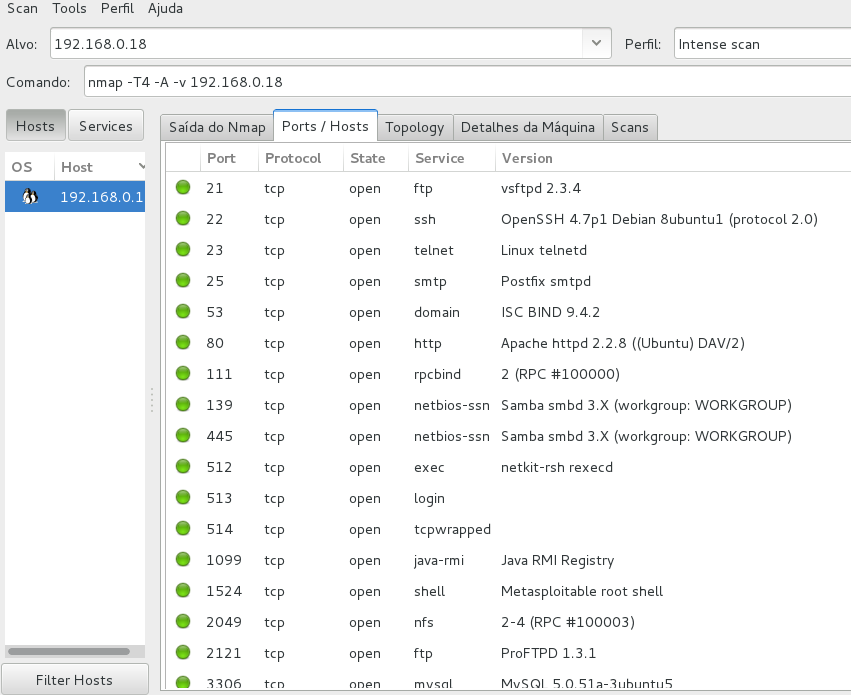
\includegraphics[width=400px, scale=1]{resource/atacante_log_port_scan}
 	 \caption{Atacante - Log do port scan(portas abertas protocolos e versão do provedor)}
  \label{fig:atacante_log_port_scan}
  \end{figure}

	\section{Flood Attack}
	\label{sec:Flood_Attack}
	Este ataque foi utilizado enviando vários pacotes na maior velocidade possível.
	Para tal, foi utilizada a ferramenta hping3 com o seguinte comando:

\begin{framed}
	hping3 -c 10000 -d 120 -S -w 64 -p 21 --flood --rand-source 192.168.0.18
\end{framed}

	Na Figura~\ref{fig:atacante_hping3} pode-se observar a utilização da ferramenta hping3 ilustrando
	os 1108443 pacote enviados, sendo que todos foram perdidos.

	 \begin{figure}[h]
 	 \centering
 	 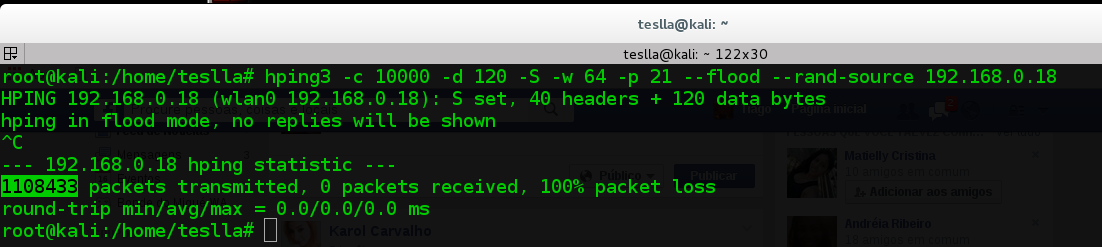
\includegraphics[width=400px, scale=1]{resource/atacante_hping3}
 	 \caption{Atacante - 1108433 pacotes enviados para a vítima}
  \label{fig:atacante_hping3}
  \end{figure}

	O servidor Snort por sua vez, detectou todos os ataque realizados. Ele identifica
	o ataque retornando a mensagem: ET FROP Spamhaus DROP Listed Traffic Inbound. O
	log dos pacotes por parte do server pode ser visto na figura \ref{fig:vitima_flood}.

	 \begin{figure}[h]
 	 \centering
 	 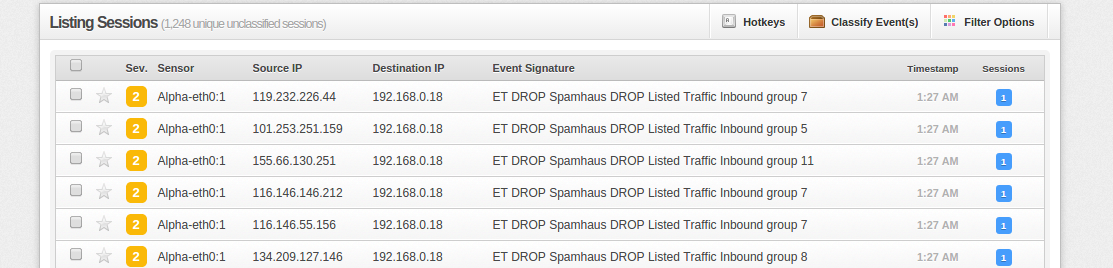
\includegraphics[width=400px, scale=1]{resource/vitima_flood}
 	 \caption{Vítima - Detecção do Ataque flood as 1:27}
  \label{fig:vitima_flood}
  \end{figure}

\section{Brute Force SSH}
\label{sec:Brute_Force_SSH}
	Os ataques citados até agora testaram apenas o serviço IDS do sistema, este agora
	será responsável por testar o serviço IPS ao perceber que o atacante está com más
	intenções para com a vítima atacante.

	O ataque utilizou a ferramenta de força bruta hydra, a qual utiliza uma lista
	de senhas para atacar um determinado servidor ssh com um determinado nome de
	usuário ou uma lista deles. Neste caso, utilizamos o usuário root, na porta 22,
	com a lista de senhas e o endereço do servidor.

	\begin{framed}
		hydra -s 22 -v -l root -P /home/teslla/Downloads/tech.lst -t 10 192.168.0.18 ssh
	\end{framed}

	Este comando foi aplicado no atacante, que iniciou os ataques. Logo o servidor
	começou a identificar os pacotes maliciosos, vistos na figura \ref{fig:ssh_vitima}.

	\begin{figure}[h]
		\centering
		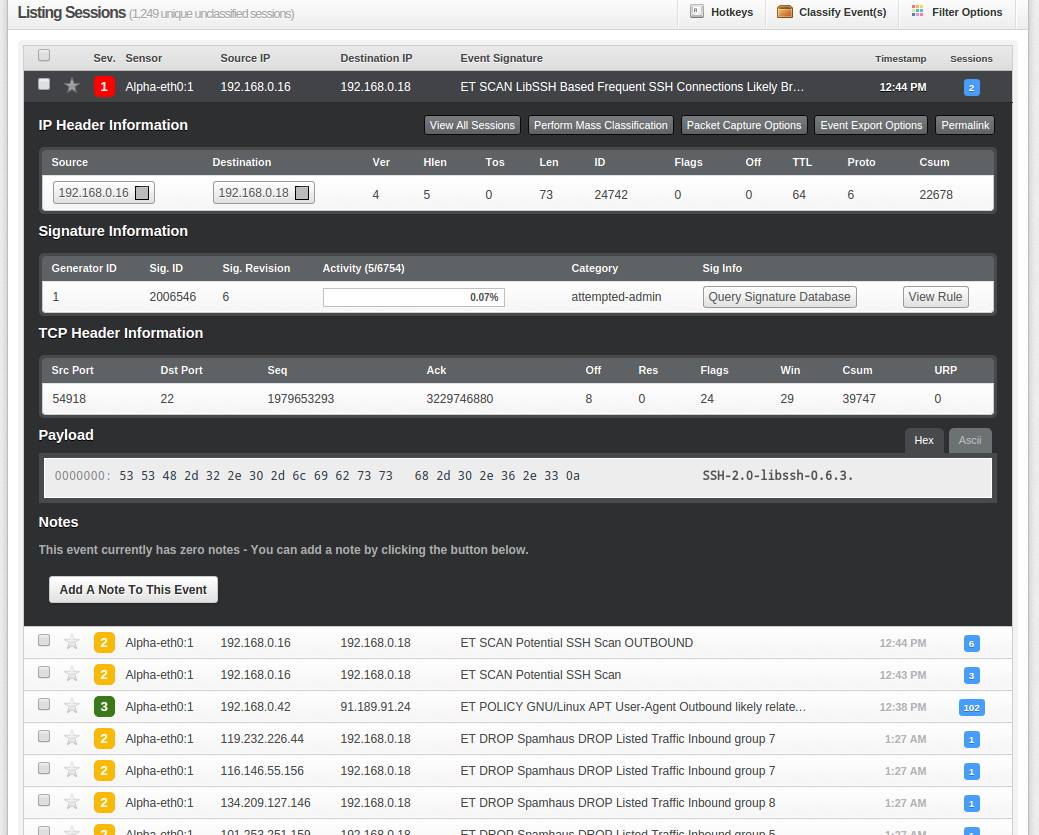
\includegraphics[width=400px, scale=1]{resource/ssh_vitima}
		\caption{Vítima - Detecção do Ataque brute force SSH}
		\label{fig:ssh_vitima}
	\end{figure}
	\newpage
 	Quando o servidor percebeu que se tratava de um ataque brute force, este bloqueou
	o tráfico advindo do atacante e o hydra ficou travado. Exemplificando o serviço
	do IPS disponível no Security Onion.
